\documentclass[tikz]{standalone}
\usepackage{amsmath,mathtools}
\begin{document}
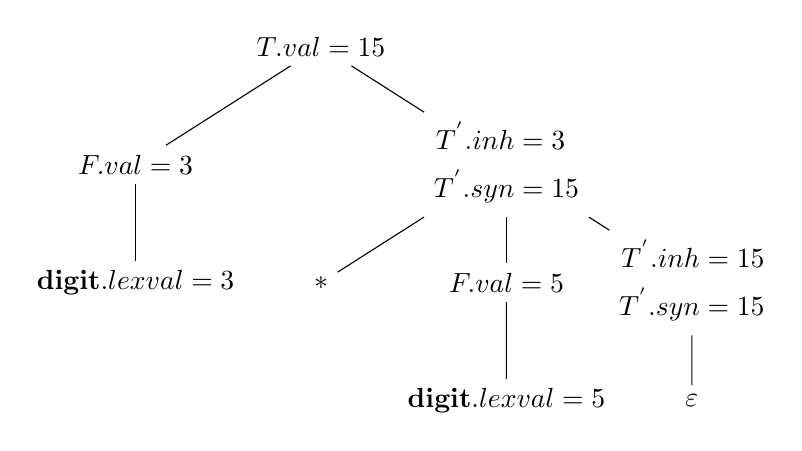
\begin{tikzpicture}[level/.style={sibling distance=13.4em/#1}]
  \node{\(T.val=15\)}
  child {
    node {\(F.val=3\)}
    child {
      node {\(\textbf{digit}.lexval=3\)}
    }
  }
  child {
    node {\(\begin{aligned} T^{'}.inh &= 3\\ T^{'}.syn &= 15 \end{aligned}\)}
    child {
      node {\(*\)}
    }
    child {
      node {\(F.val=5\)}
      child {
        node {\(\textbf{digit}.lexval=5\)}
      }
    }
    child {
      node {\(\begin{aligned} T^{'}.inh &= 15\\ T^{'}.syn &= 15 \end{aligned}\)}
      child {
        node {\(\varepsilon\)}
      }
    }
  };
\end{tikzpicture}
\end{document}
